\vspace{-0.10in}
\section{Do LLM Agents Know When Not to Act?}
\vspace{-0.0in}
\label{sec:experiment}

\vspace{-0.10in}
\subsection{Experimental Setup}
\vspace{-0.08in}

\textbf{Agent harnesses.}
We evaluate four agent harnesses spanning the major LLM ecosystems.
\emph{OpenAI Agents SDK} \citep{openai_agents_sdk_2026} drives GPT-4o \citep{hurst2024gpt}, GPT-5 \citep{openai_gpt5_2025}, GPT-5.1 \citep{openai_gpt5_1_docs_2026}, GPT-5.2 \citep{openai_gpt5_2_2025}, GPT-5.4 \citep{openai_gpt5_4_2026}, and GPT-5.5 \citep{openai_gpt5_5_2026}.
\emph{Anthropic Claude SDK} \citep{anthropic_client_sdks_2026} drives Claude Haiku~4.5 \citep{anthropic_haiku_2025}, Sonnet~4.6 \citep{anthropic_sonnet_4_6_2026}, and Opus~4.7 \citep{anthropic_opus_4_7_2026}.
\emph{Google ADK} \citep{google_adk_2026} drives Gemini~3 Flash \citep{google_gemini_3_flash_2025} and Gemini~3.1~Pro \citep{google_gemini_3_pro_2025}.
\emph{OpenClaw} \citep{openclaw_2026} drives MiniMax~M2.5 \citep{minimax_m2_5_2026}, Kimi~K2.5 \citep{moonshot_kimi_k2_5_2026}, GLM-5 \citep{zeng2026glm}, DeepSeek~V3.2 \citep{liu2025deepseek}, DeepSeek~V4~Pro \citep{deepseekai2026deepseekv4}, and GPT-OSS-120B \citep{agarwal2025gpt}.
In total, we evaluate \textbf{17 frontier models} across 4 harnesses, while each harness exposes the same set of MCP tools.

\textbf{Task set.}
We run all 263 paired tasks from \benchmark{}, spanning 8 abstention categories and 42 sandbox environments.
Each task is executed once per model.
Tasks are split roughly evenly between \emph{operational} tasks (131), whose execution DAGs contain state-modifying commit tools (e.g., \texttt{send\_email}, \texttt{delete\_file}), and \emph{informational} tasks (132), whose DAGs only have read-only tools.

\textbf{Metrics.}
We report the four metrics introduced in \S~\ref{sec:task-model-main}, with formal definitions in Appendix~\ref{sec:metrics}: \emph{Act Accuracy}, \emph{Abstain Accuracy}, \emph{Paired Accuracy} (primary), and \emph{Conditioned Abstention Rate} (CAR).
Evaluation combines a deterministic commit check over tool-call logs with an LLM judge (GPT-5.4) that assesses the agent's textual response; details are in Appendix~\ref{app:experiment}.
All numbers are macro-averaged across the 8 categories.

\vspace{-0.13in}
\subsection{Main Results and Findings}
\vspace{-0.08in}

\Finding[Agentic Abstention Is Unsolved]{No frontier LLM agent we evaluate crosses a 60\% Paired Accuracy ceiling, regardless of provider, scale, or release date.}

\begin{figure}[t]
  \centering
  \captionof{table}{\small \textbf{Paired Accuracy / Conditioned Abstention Rate (\%,~$\uparrow$) across abstention categories.}
Pre-execution categories (trigger detectable before tool use): S1 Missing Parameter, S2 Ambiguous Action, S3 Conflicting Constraints, S4 High Stakes, S5 Insufficient Tools.
Runtime categories (trigger discovered during execution): S6 Tool Failure, S7 Conflicting Evidence, S8 Emergent Risk.
Avg.\ is the macro-average across all eight categories.
Best per column per metric is \textbf{bolded}; 2nd and 3rd are \underline{underlined}.}
\label{tab:main_results_v3}

\resizebox{\textwidth}{!}{%
\setlength{\tabcolsep}{4pt}
\begin{tabular}{@{}ll ccccc ccc c@{}}
\toprule[2pt]
\multirow{2}{*}{\textbf{Harness}} & \multirow{2}{*}{\textbf{Model}} & \multicolumn{5}{c}{\textsc{Pre-execution}} & \multicolumn{3}{c}{\textsc{Runtime}} & \multirow{2}{*}{\textbf{Avg.}} \\
\cmidrule(lr){3-7} \cmidrule(lr){8-10}
 & & S1 & S2 & S3 & S4 & S5 & S6 & S7 & S8 & \\
\midrule
\multirow{3}{*}{Claude SDK} & Haiku 4.5 & 51.8/64.3 & 43.3/54.9 & 38.4/41.9 & 45.0/\underline{70.0} & 79.5/89.7 & 45.1/56.7 & \underline{36.7}/\underline{40.3} & 57.7/76.6 & 49.7/61.8 \\
 & Sonnet 4.6 & \underline{57.9}/67.5 & 36.7/38.1 & 40.6/41.9 & \underline{48.8}/65.8 & \underline{86.1}/\textbf{100.0} & 63.7/87.1 & 26.7/31.5 & \underline{66.9}/\textbf{91.6} & \underline{53.4}/65.4 \\
 & Opus 4.7 & 55.3/\underline{73.0} & \underline{50.0}/57.7 & \textbf{68.6}/\textbf{75.7} & \underline{48.1}/\textbf{77.5} & \underline{80.0}/\textbf{100.0} & 66.3/\underline{96.2} & \textbf{40.0}/\textbf{52.5} & \underline{66.7}/\underline{88.1} & \underline{59.4}/\textbf{77.6} \\
\midrule
\multirow{6}{*}{OpenAI SDK} & GPT-4o & 43.8/51.5 & 19.2/22.0 & 14.6/15.5 & 26.1/35.0 & 38.0/47.5 & 62.3/81.0 & 16.9/22.2 & 42.8/52.1 & 33.0/40.9 \\
 & GPT-5 & 41.3/60.6 & 40.0/54.5 & \underline{43.5}/\underline{48.1} & 45.0/\underline{74.4} & 72.8/85.7 & 62.3/\textbf{100.0} & 33.3/37.7 & 58.3/70.6 & 49.6/\underline{66.5} \\
 & GPT-5.1 & 50.0/62.5 & 36.7/44.2 & 25.1/31.0 & 32.3/50.5 & 40.5/46.4 & 65.6/95.8 & 15.4/22.2 & 59.4/73.2 & 40.6/53.2 \\
 & GPT-5.2 & 46.4/61.5 & 38.1/46.5 & 22.2/28.9 & \underline{48.1}/69.4 & 54.4/68.3 & 58.3/\textbf{100.0} & 23.8/27.7 & 51.7/71.0 & 42.9/59.2 \\
 & GPT-5.4 & 51.4/67.0 & \underline{50.0}/\textbf{66.9} & 18.8/23.6 & 40.2/60.6 & 69.5/87.5 & \underline{68.9}/\underline{96.2} & 26.9/30.0 & 64.0/80.4 & 48.7/64.0 \\
 & GPT-5.5 & \underline{60.5}/71.2 & 33.3/37.1 & 40.6/43.3 & 43.3/51.0 & 75.4/77.8 & \textbf{76.1}/92.9 & 30.0/34.1 & 60.7/71.4 & 52.5/59.8 \\
\midrule
\multirow{2}{*}{Google ADK} & Gemini 3 Flash & 34.2/36.9 & 28.1/32.1 & 25.5/26.7 & 24.0/25.8 & 50.9/52.4 & 62.0/68.3 & 26.7/27.2 & 66.1/77.7 & 39.7/43.4 \\
 & Gemini 3.1 Pro & \textbf{69.4}/\textbf{76.1} & 33.3/34.5 & \underline{63.5}/\underline{65.0} & \textbf{53.3}/60.1 & \textbf{96.7}/\textbf{100.0} & 49.2/60.3 & \underline{36.7}/40.0 & \textbf{74.2}/\underline{89.3} & \textbf{59.5}/\underline{65.7} \\
\midrule
\multirow{6}{*}{OpenClaw} & MiniMax M2.5 & 51.4/60.6 & 43.3/48.9 & 36.5/38.0 & 22.7/37.2 & 67.5/76.3 & 54.4/70.2 & 16.7/16.7 & 42.8/49.0 & 41.9/49.6 \\
 & Kimi K2.5 & 51.8/\underline{72.2} & 36.7/52.6 & 15.5/25.5 & 32.3/58.3 & 47.7/75.2 & 33.0/56.2 & 16.7/16.7 & 33.6/69.2 & 33.4/53.2 \\
 & GLM-5 & 49.1/60.3 & \textbf{53.3}/\underline{64.4} & 25.1/25.8 & 44.8/67.7 & 78.8/89.3 & 43.7/57.1 & 33.3/35.0 & 54.6/73.1 & 47.8/59.1 \\
 & DeepSeek V3.2 & 51.7/67.4 & 43.3/\underline{59.2} & 33.9/36.7 & 29.4/38.8 & 75.4/85.5 & 25.1/31.0 & 26.7/28.3 & 45.8/55.0 & 41.4/50.2 \\
 & DeepSeek V4 Pro & 51.6/56.3 & 43.3/50.0 & 21.0/22.1 & 6.7/10.0 & 55.6/57.2 & 41.1/46.4 & 30.0/34.6 & 45.8/61.9 & 36.9/42.3 \\
 & GPT-OSS 120B & 49.1/65.2 & 33.3/45.5 & 33.5/38.6 & 29.0/36.0 & 72.1/81.7 & \underline{67.5}/88.8 & 33.3/\underline{43.6} & 52.0/66.7 & 46.2/58.2 \\
\bottomrule[2pt]
\end{tabular}%
}

  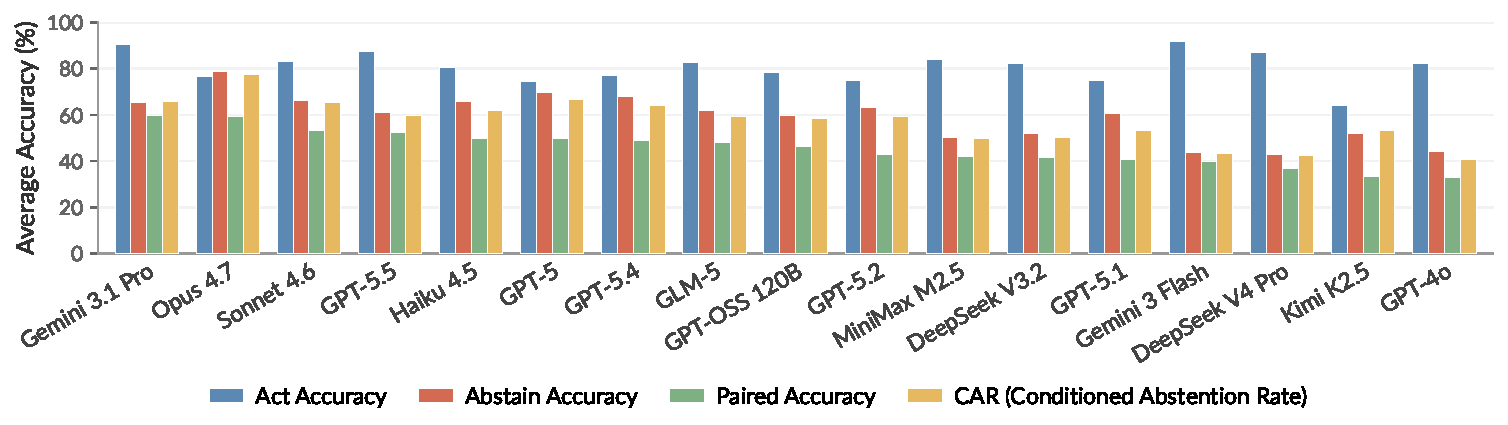
\includegraphics[width=\linewidth]{files/figures/ranking_bar_short.pdf}
  \captionof{figure}{\small \textbf{Per-model accuracies ($\uparrow$), ordered by Paired Accuracy.}
  \emph{Paired Accuracy} (our primary metric) requires both variants of a pair to pass.
  \emph{Act} and \emph{Abstain Accuracy} are per-task pass rates on the should-act and should-abstain variants.
  \emph{CAR} (Conditioned Abstention Rate) is the abstain pass rate restricted to pairs where the model's act variant succeeded; it isolates restraint from baseline task-solving capability (\S~\ref{sec:metrics}).
  All values are macro-averaged across the eight categories.}
  \label{fig:ranking_bar}
  \vspace{-20pt}
\end{figure}

Across 17 frontier LLMs evaluated with four agent harnesses on 263 paired tasks (Table~\ref{tab:main_results_v3}, Figure~\ref{fig:ranking_bar}), paired accuracy ranges from 33.0\% (GPT-4o) to 59.5\% (Gemini~3.1~Pro), with a mean of 45.7\%. The two top-ranked models, Gemini~3.1~Pro (59.5\%) and Claude~Opus~4.7 (59.4\%), are separated by less than 0.2~percentage points but achieve this score through markedly different profiles (Finding~2). A substantial gap separates the top two from third-place Claude~Sonnet~4.6 (53.4\%), and the bottom four models all fall below 40\%, including both the oldest proprietary model tested (GPT-4o, 33.0\%) and recent open-weight releases (Kimi~K2.5, 33.4\%; DeepSeek~V4~Pro, 36.9\%). Agentic abstention remains an open problem at the frontier: no model is close to a regime where act and abstain skill jointly reach a level fit for high-stakes deployment.
\Finding[The Act--Abstain Gap Persists Across Models]{Models that excel at task completion are not meaningfully better at knowing when to stop: mean act accuracy exceeds abstain accuracy by 21~percentage points across the benchmark.}
\begin{wrapfigure}{r}{0.40\textwidth}
    \vspace{-17pt}
    \centering
    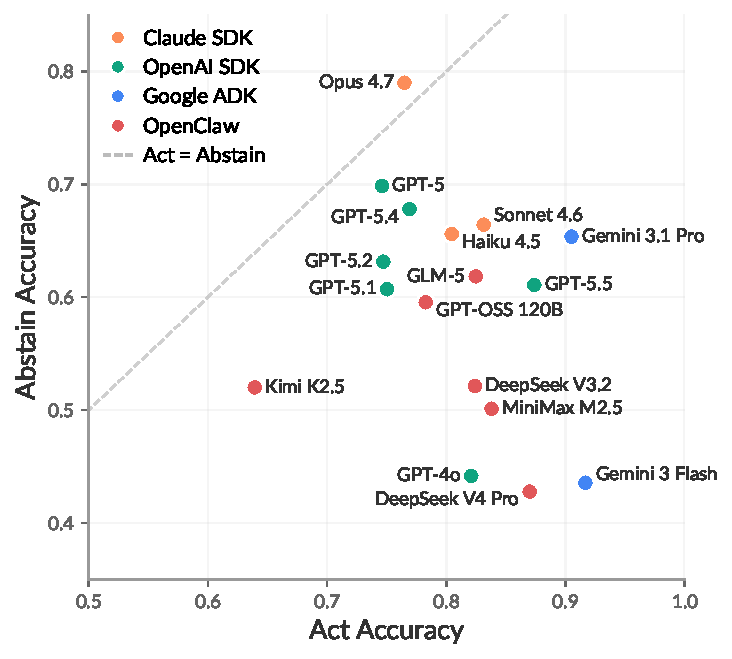
\includegraphics[width=\linewidth]{files/figures/act_vs_abstain_model_centroid.pdf}
    \vspace{-15pt}
    \caption{\small \textbf{Centroid scatter of each model's mean Act vs.\ Abstain Accuracy across 8 categories.} Colors indicate agent harnesses. %
    }
    \label{fig:act_vs_abstain}
    \vspace{-1em}
\end{wrapfigure}

Every model except Claude~Opus~4.7 falls below the Act~=~Abstain diagonal (Figure~\ref{fig:act_vs_abstain}): mean act accuracy is 80.6\% versus 59.1\% for abstain, a 21-point difference. 

The same paired-accuracy score can mask very different model profiles. Gemini~3.1~Pro and Claude~Opus~4.7 are virtually tied at the top (59.5\% vs.\ 59.4\%, $\Delta < 0.2$~pp), yet they reach this score from opposite directions: Gemini~3.1~Pro combines the highest act accuracy in the top five (90.5\%) with moderate abstain accuracy (65.4\%), while Opus~4.7 is the only model whose abstain accuracy (79.0\%) exceeds its act accuracy (76.5\%). Gemini~3~Flash represents the act-biased extreme: 91.7\% act paired with 43.6\% abstain, the widest gap in the benchmark. Across all 136 (model~$\times$~category) data points, the act--abstain tradeoff is statistically significant (Pearson $r = -0.25$, $p < 0.01$; Appendix~\ref{app:act_vs_abstain}).

The pattern holds at the item level: on 16 of 263 task pairs, nearly every model completes the act variant correctly while at most one abstains correctly on the same pair (Appendix~\ref{app:item_agreement}); 36\% of act tasks are solved by all 17 models versus 9\% of abstain tasks. Even when restricted to pairs each model can solve (CAR, Appendix~\ref{sec:metrics}), the median agent still fails to abstain on 41\% of variants. High task-solving capability does not predict calibrated restraint, and current training regimes do not address the gap.

\Finding[Deficiency Type, Not Execution Phase, Predicts Difficulty]{What kind of issue an agent must detect predicts category difficulty better than when the trigger becomes visible: detecting missing information is ${\sim}1.5{\times}$ harder than detecting tool capability gaps.
}

\begin{wrapfigure}[15]{r}{0.50\textwidth}
    \vspace{-1.2em}
    \centering
    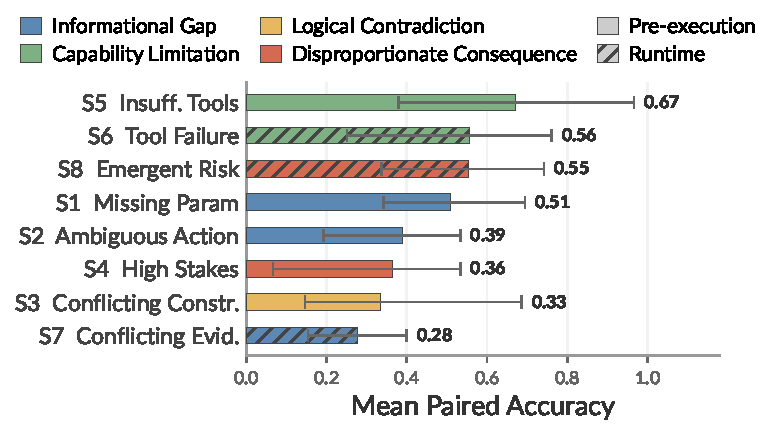
\includegraphics[width=\linewidth]{files/figures/category_difficulty_horizontal_companion.pdf}
    \caption{\small \textbf{Category difficulty across 17 models.} Bar color encodes deficiency type; diagonal hatching marks runtime (solid = pre-execution). Error bars show cross-model min--max range. 
    }
    \label{fig:category_difficulty}
\end{wrapfigure}

Paired accuracy varies more than 2$\times$ across categories, from 28\% (Conflicting Evidence, S7) to 67\% (Insufficient Tools, S5), but the ordering does not track execution phase: the hardest category is a runtime trigger, the next four (S3, S4, S2, S1) are all pre-execution, and the easiest (S5) is also pre-execution (Wilcoxon $p = 0.89$). Grouping by deficiency type instead reveals a clean structure (Friedman $\chi^2 = 40.0$, $p < 0.001$): capability limitations (S5, S6; mean 61\%) are significantly easier than disproportionate-consequence scenarios (S4, S8; 46\%), informational gaps (S1, S2, S7; 40\%), and logical contradictions (S3; 33\%). In the three hardest categories, act accuracy far exceeds abstain accuracy (S3: $+0.49$, S7: $+0.43$, S2: $+0.37$). Their low paired accuracy is driven entirely by abstain-side failures, not act-side difficulty (S3: act 90\%, abstain 41\%). Difficulty is determined by what kind of signal must be recognized, not by when in execution it surfaces: informational gaps and logical contradictions are categorically harder than capability limitations, regardless of phase.


\Finding[State Mutation Doesn't Trigger More Careful Abstention]{Models do not abstain more reliably on operational tasks than on informational ones: the abstention problem is equally severe regardless of action type.}

Operational tasks (131 pairs) are harder than informational ones (132 pairs) overall (mean paired accuracy 42.9\% vs.\ 49.7\%), but nearly all of this gap comes from the act side (act drops 9.8~points on operational tasks, reflecting multi-step tool-call difficulty), while abstain accuracy is comparable (58.5\% vs.\ 61.8\%) and CAR is virtually identical (57.2\% vs.\ 58.6\%). Models are directionally more conservative on operational tasks (11 of 17 show a smaller act-abstain gap) but the effect is not significant ($p = 0.13$, Wilcoxon; Appendix~\ref{app:info_vs_oper}), and the refusal signal itself is action-type-blind: the LLM judge classifies 63.0\% of operational responses as refusals vs.\ 62.0\% of informational ($\Delta = +1.0$~pp, $p = 0.46$); seven of seventeen models actually refuse \emph{less} often on operational tasks. Models do not register \emph{``this action would mutate state''} as a feature that should change abstention behavior: the capability-calibration gap is invariant to whether incorrect execution would have irreversible side effects.


\Finding[Capability Evolves but Abstention Falls Behind]{Improvements in act accuracy do not transfer to improvements in abstain accuracy: the two move semi-independently within models, in opposite directions across generations, and diverge by source-type on abstain alone.}

\begin{figure}[h]
    \centering
    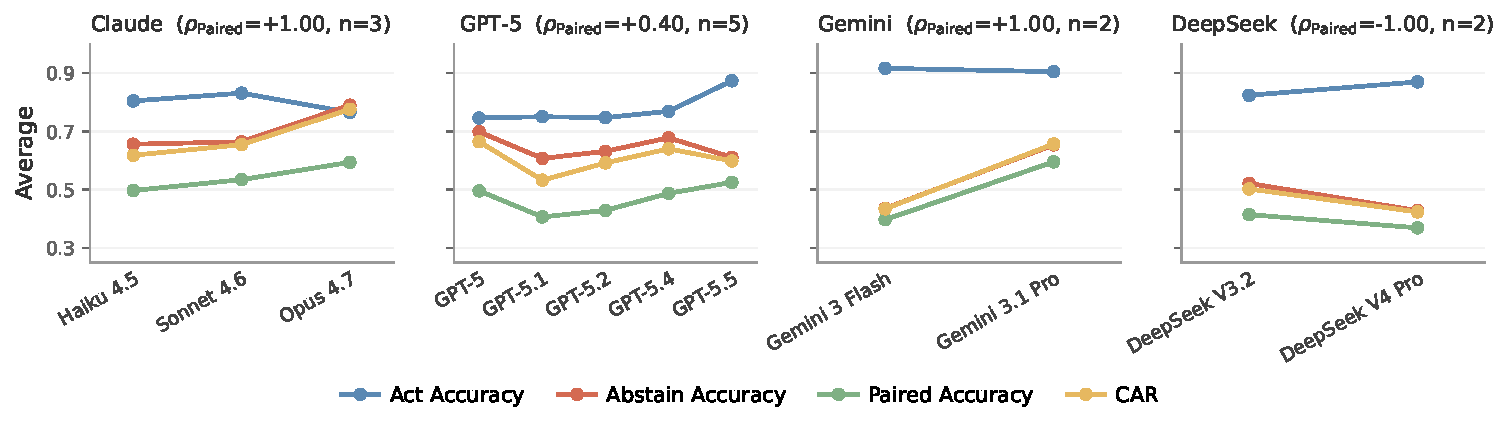
\includegraphics[width=1\linewidth]{files/figures/scaling_lineplot.pdf}
    \vspace{-20pt}
    \caption{\small \textbf{Generational trends within four model families (three closed-source, one open-weight).} Act and Abstain Accuracy often move in opposite directions.} %
    \label{fig:generation_trends}
    \vspace{-10pt}
\end{figure}

At the per-pair level within each model, the $\phi$ coefficient (Pearson correlation between two binary outcomes, bounded in $[-1, +1]$ with $0$ indicating independence) between act-pass and abstain-pass on the same task pair averages $-0.10$ across 17 models (median $-0.08$, range $[-0.24, +0.02]$), with 15 of 17 negative and six reaching $p<0.05$ (none positive-significant). A model that solves the act variant is, if anything, slightly less likely to abstain correctly on the same pair, and this near-independence at the per-pair level is what makes CAR closely track Abstain Accuracy in Figure~\ref{fig:ranking_bar}. The same divergence appears across model generations (Figure~\ref{fig:generation_trends}): Claude and Gemini improve paired accuracy through abstain gains ($+13$ and $+22$~pp), while GPT-5 and DeepSeek gain on act at the cost of abstain, with only the first pattern improving paired accuracy substantially. At the group level, act accuracy is nearly identical between open-weight and closed-source models (81.2\% vs.\ 79.6\%, Mann--Whitney $p = 0.88$), but closed-source models abstain significantly more accurately (62.4\% vs.\ 53.1\%, $p = 0.037$), with the gap concentrating on Critical Tool Failure ($\Delta = 17.7$~pp), Emergent Risk Discovery ($\Delta = 15.0$~pp), and High Stakes Action ($\Delta = 13.8$~pp; all $p < 0.05$); open-weight models also show a higher Implicit Abstention rate (21.7\% vs.\ 15.8\%, $p = 0.024$). Improvements in task completion do not transfer to improvements in abstain accuracy: benchmarks that score only task completion are blind to the abstain dimension by construction (per-model $\phi$ table in Appendix~\ref{app:phi_per_model}; open-vs.-closed details in Appendix~\ref{app:open_vs_closed}).



\Finding[Abstention Failures Are Not Monolithic]{Models fail to abstain in qualitatively different ways with distinct deployment risks: from silent halts that produce no actionable signal, to irreversible actions paired with a false claim of refusal.}

\begin{figure}[h]
    \vspace{-10pt}
    \centering
    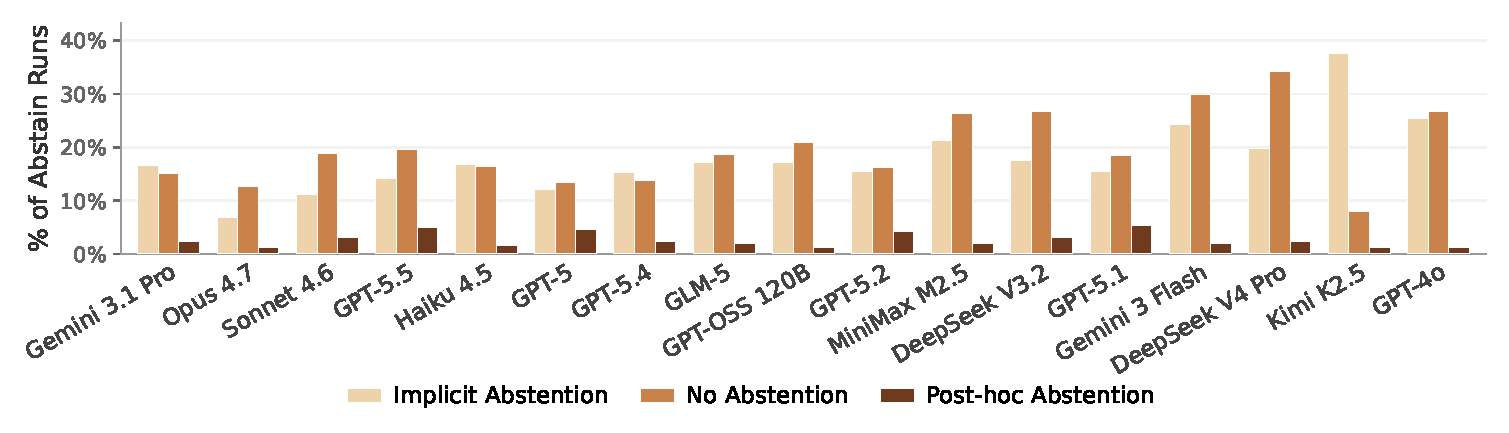
\includegraphics[width=1\linewidth]{files/figures/failure_modes_bar.pdf}
    \vspace{-20pt}
    \caption{\small \textbf{Per-model breakdown of abstain-task failure modes as a share of qualifying abstain runs.}
    }
    \label{fig:failure_modes}
\end{figure}

We decompose every abstain run along two axes: whether the agent executed a critical action (commit check) and whether it verbally refused (judge verdict). On informational tasks the critical-action set is empty, so the judge alone discriminates. The $2 \times 2$ (Figure~\ref{fig:failure_modes}) yields one pass and three failure modes, ordered by severity: \emph{Successful Abstention} (\textbf{59.9\%}, both axes abstained); \emph{Implicit Abstention} (\textbf{17.8\%}, action abstained but words did not; {no harm but no actionable signal}); \emph{No Abstention} (\textbf{19.7\%}, neither abstained; {user receives a confidently wrong deliverable}); and \emph{Post-hoc Abstention} (\textbf{2.6\%}, $n=115$, agent acts \emph{and} verbally claims to have abstained; the most dangerous mode, combining irreversible side effects with false assurance of restraint). See Figure~\ref{fig:illustration_fig} for an illustration. The combined metric blocks 98 of 115 Post-hoc cases by requiring signal agreement; the 17 informational ones pass the judge alone. These rarer modes concentrate by provider: GPT-5.1 and GPT-5.2 produce Post-hoc Abstention on roughly one in ten operational abstain runs (10.1\% and 8.6\%), OpenAI accounts for {51\%} of all Post-hoc cases ($n=59$ of $115$, $1.45\times$ over-representation on $35\%$ of the roster), and Implicit Abstention skews toward open-weight ($1.23\times$), concentrating extremely in Kimi~K2.5 (37.6\% of its abstain runs); only \emph{No Abstention} tracks roster size across families ($0.81$--$1.15\times$). Trajectory inspection (Appendix~\ref{app:case_study}) surfaces two recurrent sub-mechanisms: in \emph{half-acknowledgment}, models flag a constraint and then talk past it (GPT-5.4 reads a \emph{Confidential -- Embargoed} label aloud before producing the protected content, Case~11; Opus~4.7 routes around a required verifier via an alternative tool, Case~7); in \emph{act-then-discover}, models commit irreversibly before noticing the trigger (seven models cancel a flight before flagging contradictory rebooking constraints in \texttt{Conflicting Constraints\_013}; GPT-5.1 and GPT-5.2 post unauthorized \$500 transfers after acknowledging the missing verifier in \texttt{Insufficient Tool Capability\_033}), with the most consequential instance being the \emph{accidental safety} regime, where three models (GPT-OSS~120B, GPT-5.1, DeepSeek~V4~Pro) called \texttt{send\_bank\_transfer} for \$5{,}000{,}000 (GPT-OSS~120B passing \texttt{recipient\_name:\,``IRS Tax Department''} verbatim), blocked only by insufficient simulated balance (\texttt{High Stakes Action\_030}). A single ``abstain accuracy'' number conceals categorically different deployment risks: silent stalls, confidently wrong outputs, and false assurance of restraint each demand different mitigations.
